\chapter{Implementation}
This chapter will explain how the described concept has been implemented.
First an overview of the concept and then the main parts of the software in more
detail.
The trackable marker is attached to the ultrasound probe. The marker is
detectable by the tracking camera and enables the camera to determine the
position and orientation of the ultrasound probe. The probe on its own will
create an ultrasound image. Then the sampled ultrasound image and pose will be
post processed as a pair in the computer. In the software, depending on the
actual state of the surgery, the use of the two will be different.

\begin{figure}[H]
  \centering
 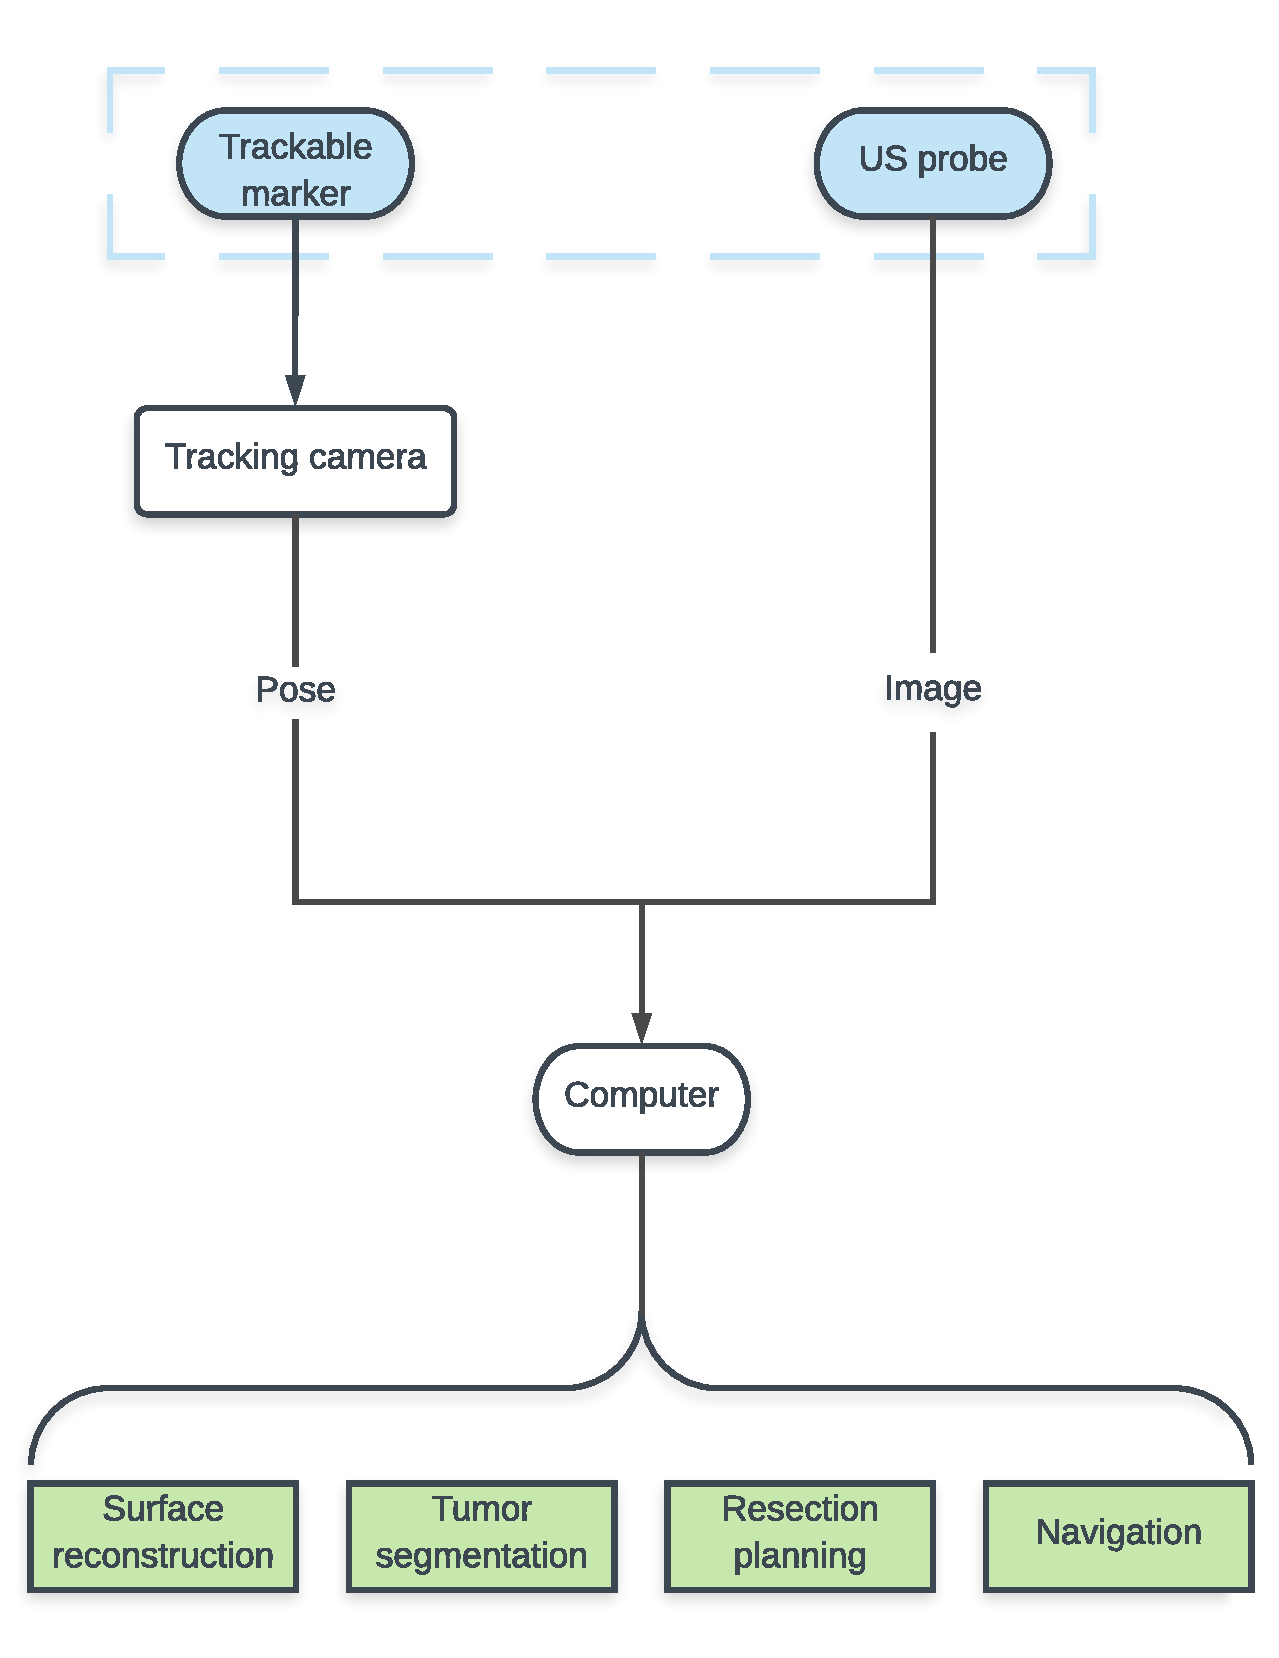
\includegraphics[width=0.65\textwidth]{FirstFlowChart}
  \caption{The way of the ultrasound image and the corresponding pose to the
    computer and later to the different parts in the software.}
  \label{fig:FirstFlowChart}
\end{figure}

\section{Surface Reconstruction}
While the surgeon is scanning the surface, the software in the background
filters out unusable positions. An image pose pair has to take two hurdles to
become accepted in the group of surface points. The image has to prove that it
arised from the liver surface and the position has to have a similar distance to
its neighbors as its neighbors to it. 
When enough points are sampled, the reconstruction of the surface will be
carried out.
\begin{figure}[H]
  \centering
 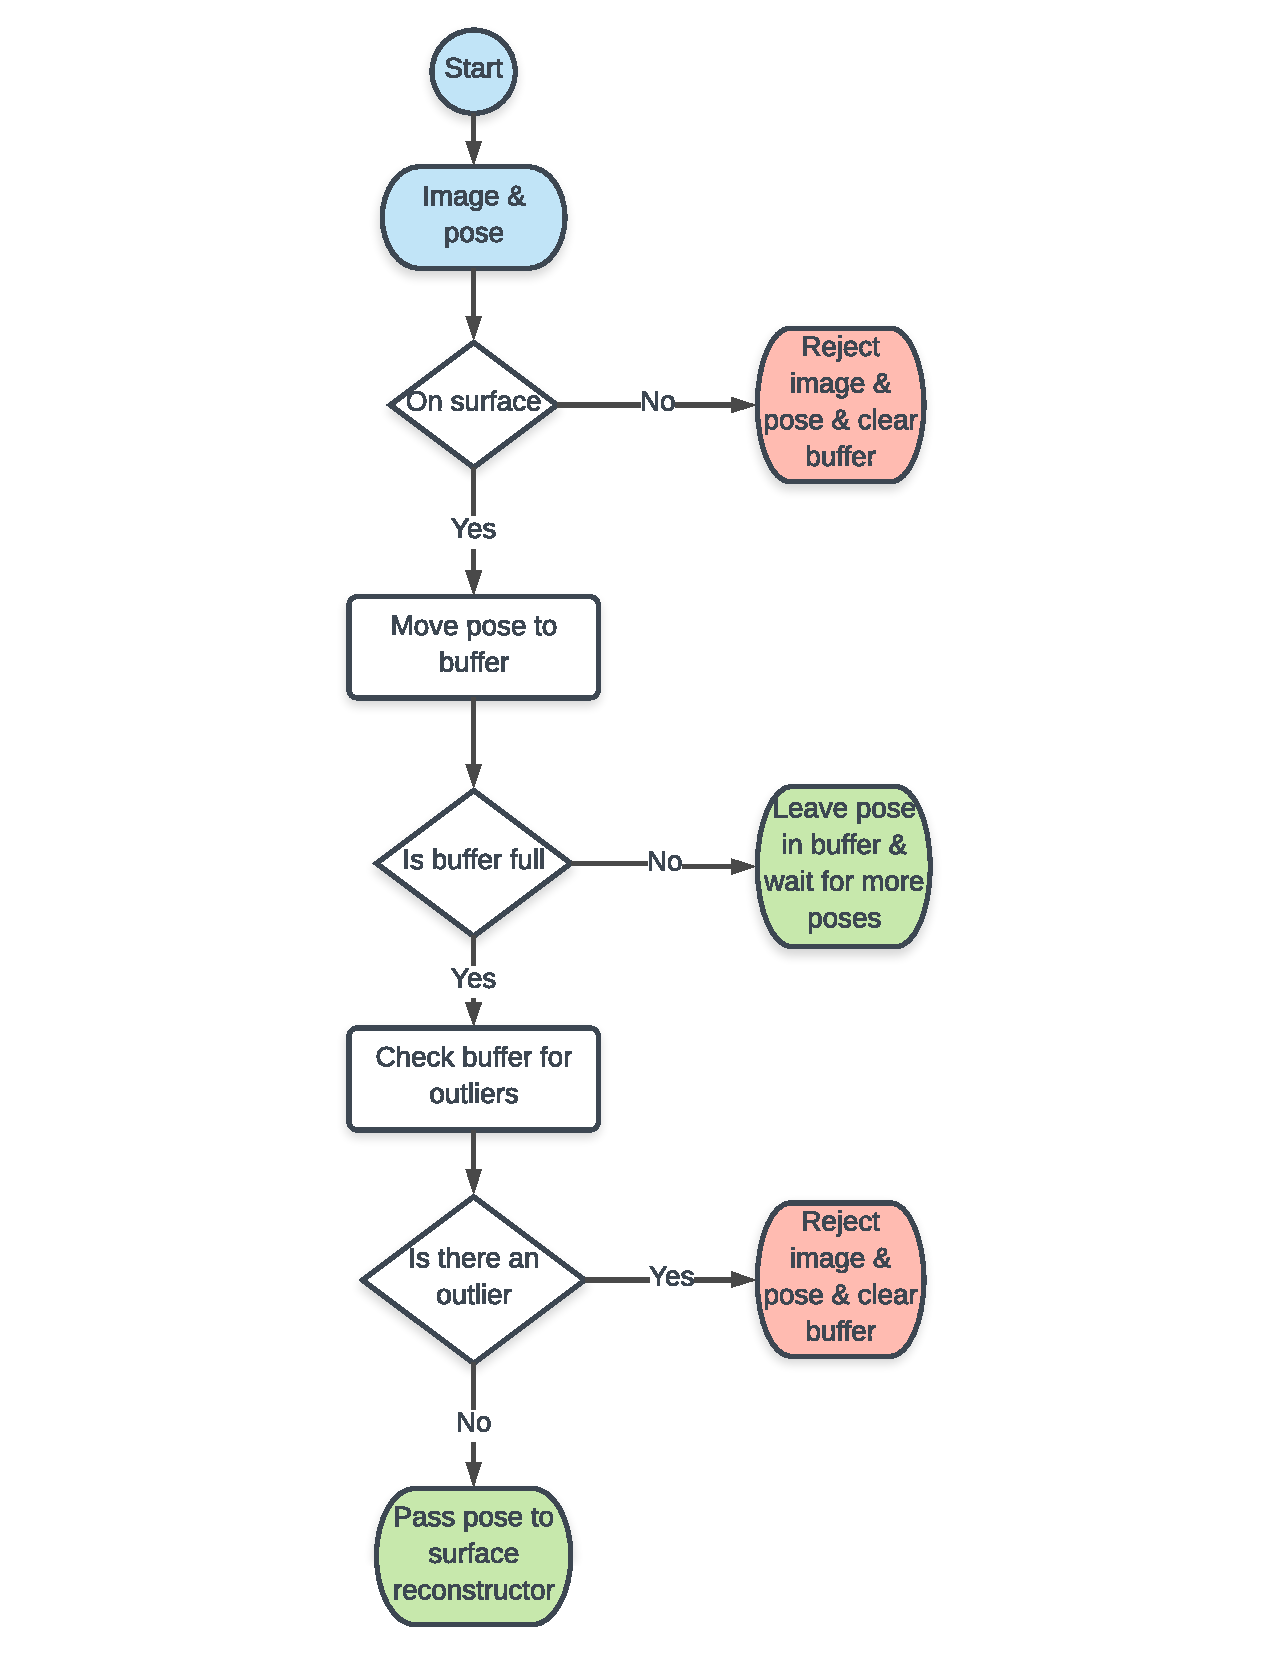
\includegraphics[width=0.65\textwidth]{SecondFlowChart}
  \caption{The way of the image and its pose if the surgeon is scanning the
    surface.}
  \label{fig:SecondFlowChart}
\end{figure}

\subsection{Surface contact detection}
For an image pose pair, the first step to pass is the contatct detection. Only
the ultrasound image is needed in this step. 

\begin{figure}[H]
  \centering
  \minipage{0.32\linewidth}
  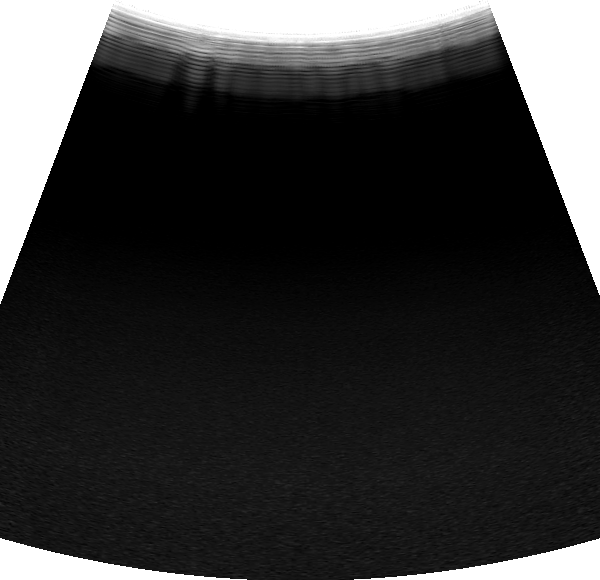
\includegraphics[width=\linewidth]{contact_no}
  \endminipage
  \hfill
  \minipage{0.32\linewidth}
  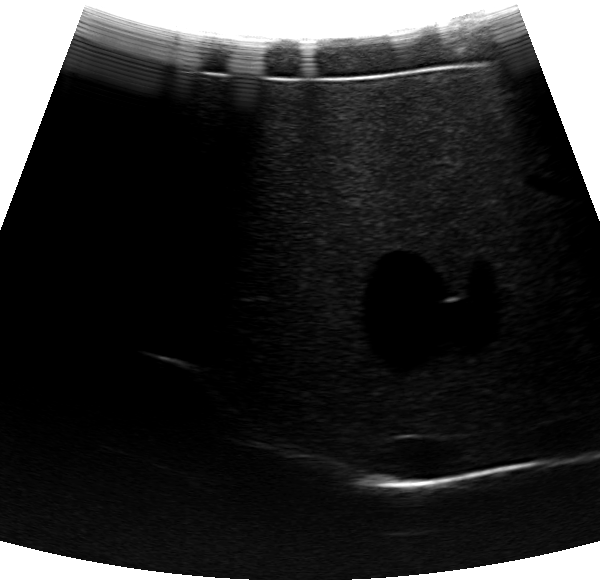
\includegraphics[width=\linewidth]{contact_difficult}
  \endminipage
  \hfill
  \minipage{0.32\linewidth}
  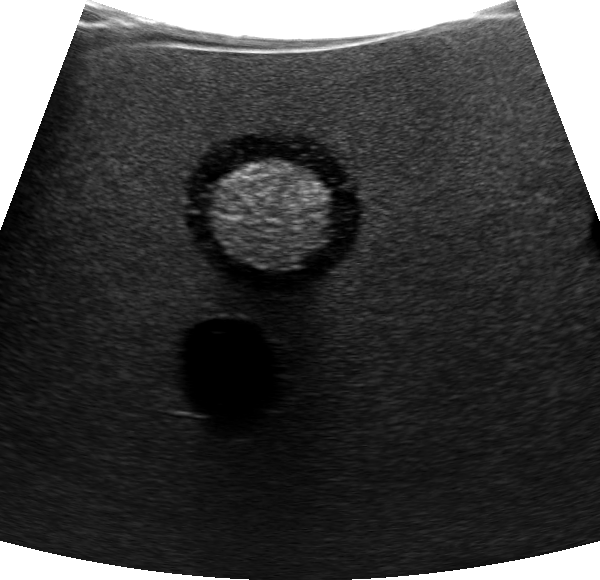
\includegraphics[width=\linewidth]{contact}
  \endminipage
  \hfill 
 \caption{Three ultrasound images from left to right: No contact with the liver,
   difficult to decide (In this case it would be contact because the middle part
   of the image shows contact), contact with the liver}
  \label{fig:contactVSnocontact}
\end{figure}

A classifier detects whether the US probe has contact to the liver or not. Therefore, a support vector machine (SVM) was trained with US images
from the phantom and from previous navigated liver surgeries. The SVM was trained to
classify the image into ``no surface contact'' (left) and ``surface contact'' (middle and right).
The images were labelled as "surface contact" if at least 50\% and the center had contact
to the surface (Figure 6.4 middle). The classifier takes into account that US waves are
reflected at the US probe-air interface when the US probe has no contact to the liver and
therefore no image is formed. The features for the classifier were: mean, median, minimum,
maximum, variance, skewness and kurtosis of the pixel values. All features are calculated
on the upper half of the image. For training, a set of 2'311 images (1'056 with contact, 1'255
without contact) were used. The training data was composed of images from a phantom
(88\%) and images from previous navigated liver surgeries (12\%). All computations were
performed using the SciPy software package. When the image is classified as ``surface contact'', then the position of the pose is stored
into the buffer. The buffer has a capacity of 10 positions. When
the addition of the actual pose leads to a full buffer, the buffer is
tested for outliers.
Each time a ``no surface contact'' image is classified and the positions buffer
is not empty it gets cleard.
\subsection{Outlier removal}
To find outliers in the current buffer the local
outlier factor is calculated for each position. 

\subsubsection{Local outlier factor}
The local outlier factor is a numerical value that describes the local density
of a position compared to its k-nearest neighbors (Figure
\ref{fig:lofExample}).

\begin{figure}[H]
  \centering
 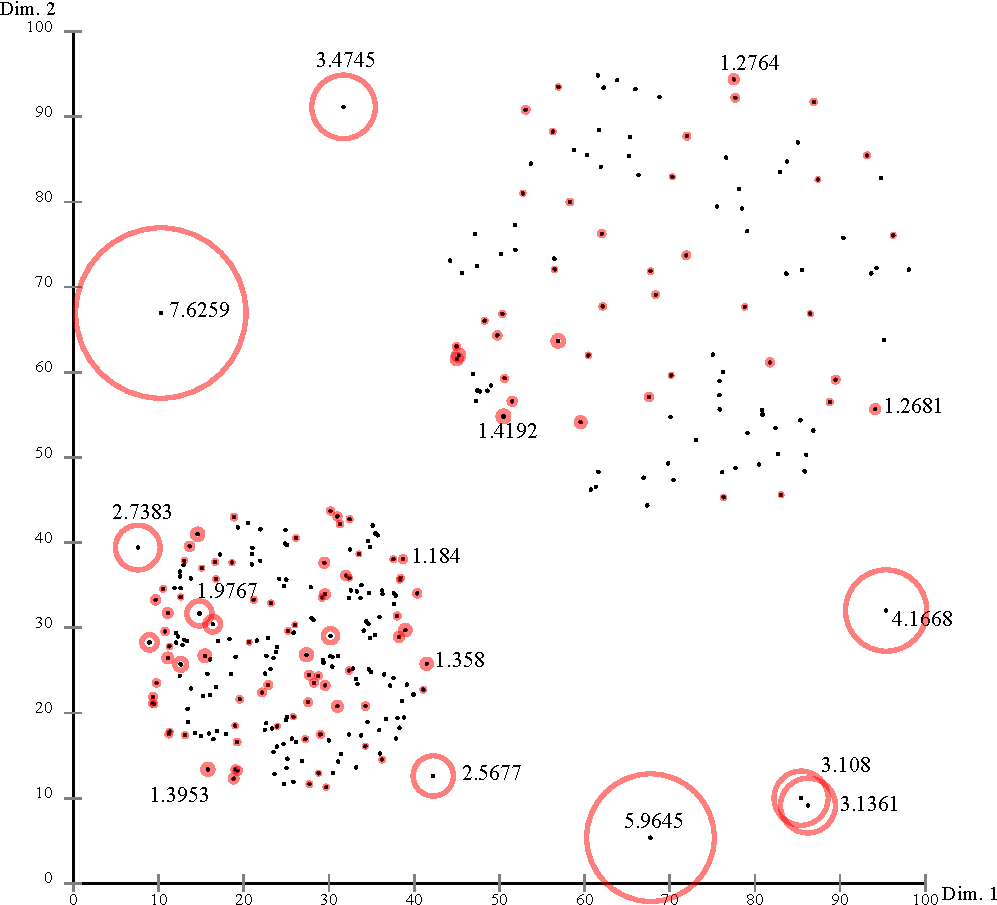
\includegraphics[width=0.6\textwidth]{lofExample}
  \caption{Example of the local outlier factors in a two dimensional pointcloud \cite{pictureLOF}.}
  \label{fig:lofExample}
\end{figure}

Five steps can be separeted to find the LOF of one position.
\begin{enumerate}
  \item{For each point calculate the distance to all the other points in the buffer}
  \item{For each point find the distance to his k-nearest neighbor $\rightarrow$
      \textit{k-distance}}
  \item{Find the \textit{reachability distance} from the k-nearest neighbors
      of each point to it self}
  \item{Calculate the \textit{local reachability density} for all points}
  \item{Calculate the \textit{local outlier factor}}
\end{enumerate}
The \textit{reachability distance} of point $A$ from another point $B$ is defined:
\begin{gather*}
  \mbox{reachability-d}_k(A,B)=\max\{\mbox{k\_d}(B), \mbox{d}(A,B)\}
\end{gather*}
The \textit{k-distance} of point $B$ depends on its k-nearest neighbors
and does not need to include point $A$.
But the actual distance between point $A$ and $B$ depends on only $A$
and $B$. The larger of the two will be the \textit{reachability distance} of
point $A$ from point $B$.

The \textit{local reachability density} of a point $A$ describes its neighborhood
and is defined by:
\begin{gather*}
  \mbox{LRD}(A):=1/\left(\frac{\sum_{B\in kNN(A)}\mbox{reachability-d}_k(A, B)}{|kNN(A)|}\right)
\end{gather*}
In words this is the inverse of the sum of the \textit{reachability distances} of point $A$
from its k-nearest neighbors devided by $k$.

Finally the \textit{local outlier factor} of a point $A$ indicates how his
neighborhood compares with the neighborhoods of his k-nearest neighbors. The LOF
of $A$ is defined by:
\begin{gather*}
  \mbox{LOF}(A):=\frac{\sum_{B\in kNN(A)}\frac{\mbox{LRD}(B)}{\mbox{LRD}(A)}}{|kNN(A)|}
\end{gather*}
If the neighborhood of $A$ is very similar to the neighborhoods of its k-nearest
neighbors, the LOF is close to 1. If its neighborhood is less dense than the
neighborhoods of his k-nearest neighbors, the LOF becomes larger than 1. If its
neighborhood is more dense than the neighborhoods of his k-nearest neighbors,
the LOF becomes lower than 1. \\
 \\
If an outlier is found in the buffer, the whole buffer is cleared. In the case
that no outlier is found, the oldest pose in the buffer gets moved into the
point collection to reconstruct the surface from.
\subsection{Reconstruction Parameters}
Finally there is a pointcloud with all the collected positions. This pointcloud
will be used as input for the surface reconstruction algorithm by Hoppe
\cite{hoppe1992surface}. The algorithm consists
of three phases. From an unorganized set of points, phase 1 constructs an
initial dense mesh. Starting with the dense mesh created in phase 1, phase 2
reduces the number of faces and improves the fit to the data points. In phase 3,
the surface representation is changed from a piecewise linear one (meshes) to a
piecewise smooth one. For the computations the implementation in VTK
(SurfaceReconstructionFilter) was used. The two main parameters of this
reconstruction algorithm have been optimized by applying the grid search method.
\subsubsection{Grid search for parameter optimization}
The \textit{neighborhood size} and the \textit{sample spacing} are the variable
parameters of the used surface reconstruction algorithm. The \textit{neighborhood size}
specifies the number of neighbors each point has. These neighbors are used to
estimate the local surface orientation. The \textit{sample spacing} sets the
spacing of a 3D sampling grid.
To find the optimal values to use in the algorithm with the point cloud data produced in the
experiment described in section \ref{sec:SurfaceReconstructionAccuracy}, a
first, rough grid search has been done to find the range of interest
of the two parameters. The same data was then used to do a second, more dense
grid search over the range of interest (Figure \ref{fig:gridSearchResultMean} and
\ref{fig:gridSearchResultSTD}). For each parameter setting, the average distance from the
reference points to the reconstructed surface was calculated.
\begin{figure}[h]
  \centering
 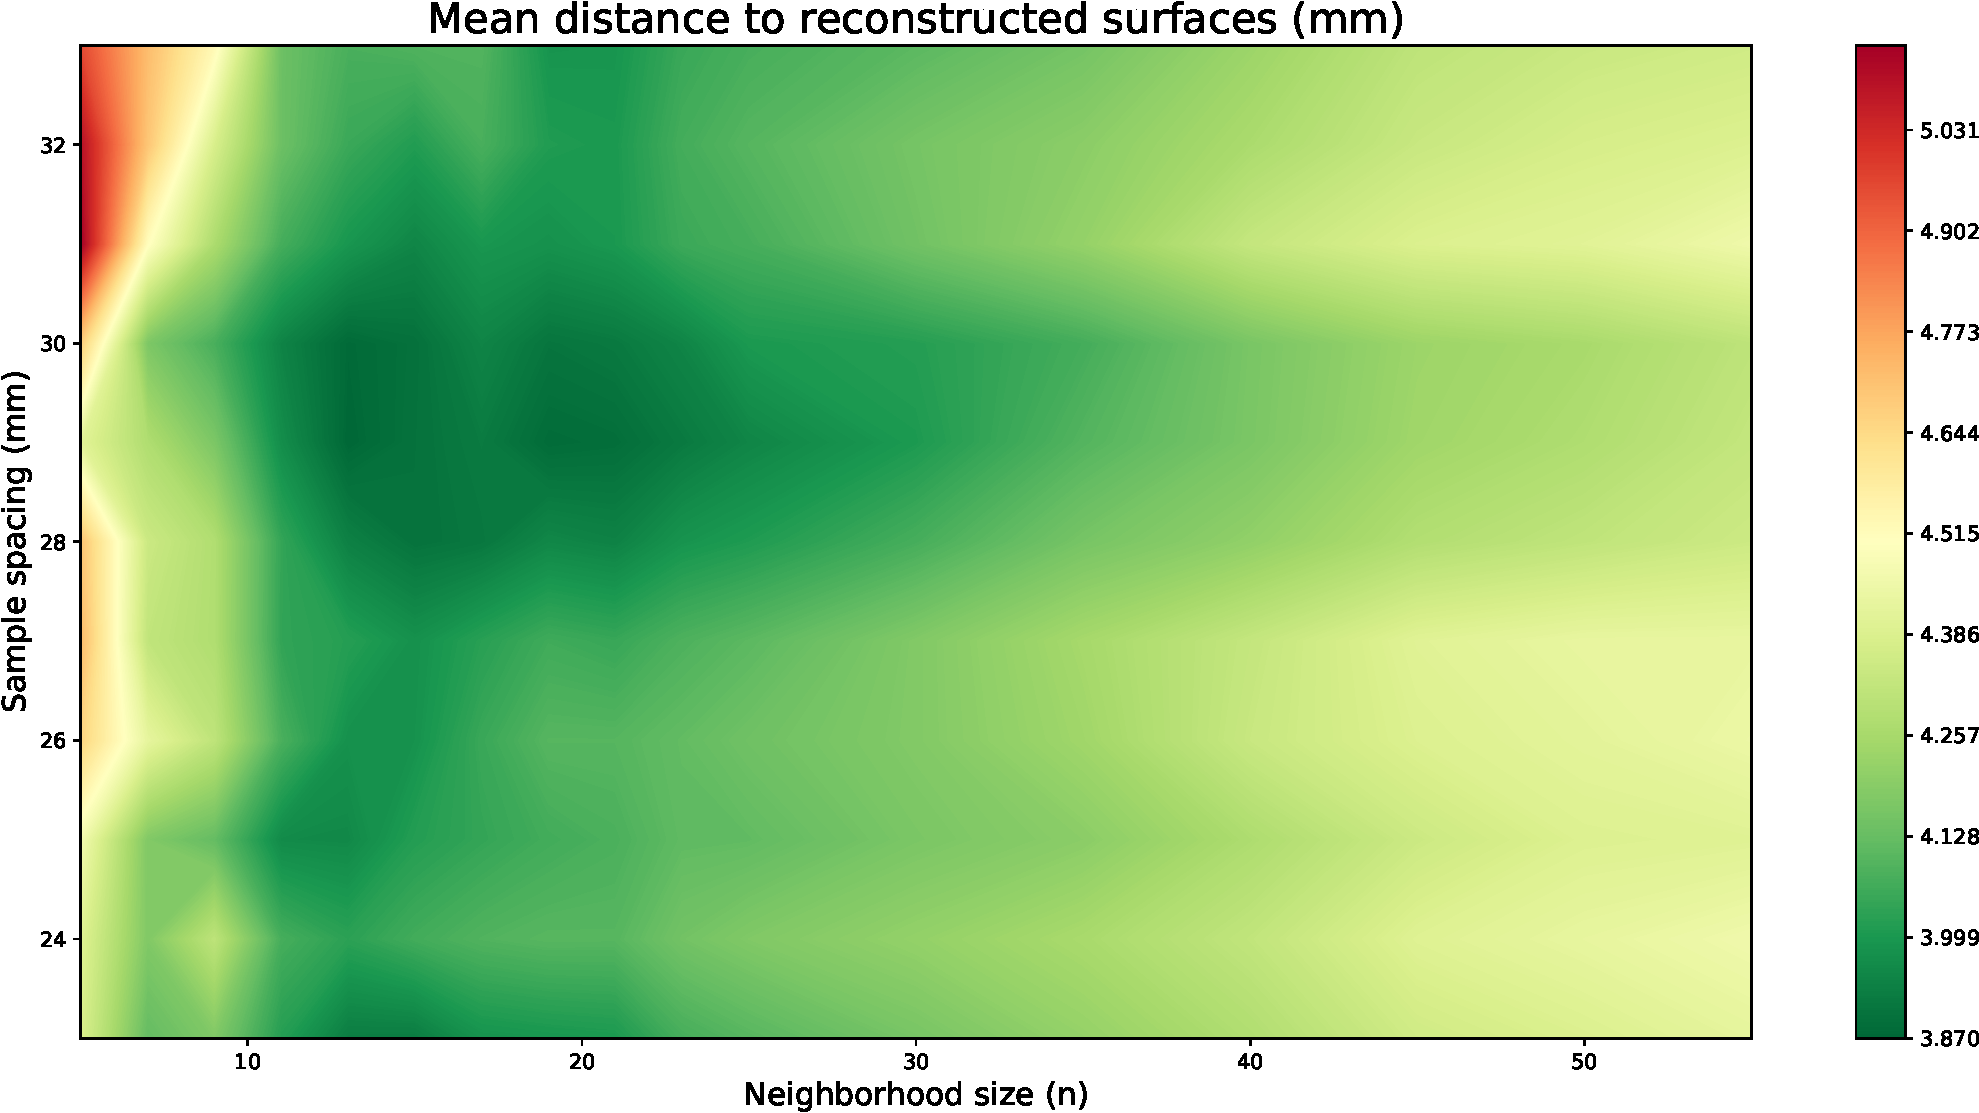
\includegraphics[width=0.9\textwidth]{gridSearchResultMeanCrop}
  \caption{This contour plot shows the mean distance calculated over 10
    differently sampled point collections. All point collections represent the
    surface of the same liver phantom.}
  \label{fig:gridSearchResultMean}
\end{figure}
The found mean distance varies from 5.1 mm to 3.9 mm. Neighborhood sizes smaller
than 8 show an increase of the mean distance for sample spacings larger than 25
mm. Neighborhood sizes over 30 seem to increase the mean distance also.
The standard deviation of the mean varies between 6.1 mm and 4.6 mm. These high
deviations result mostly from the boarder part of the reconstructions where the
reference points are more than 2 cm away from the surfaces (see section
\ref{sec:SurfaceReconstructionAccuracy}). One can say the standard deviation of
the mean decreases together with the neighborhood size used for the
reconstruction. But this is only true for neighborhood sizes larger than 13.
Because from neighborhood size 13 till 10 the standard deviation increases not
till then it decreases again. 
\begin{figure}[h]
  \centering
 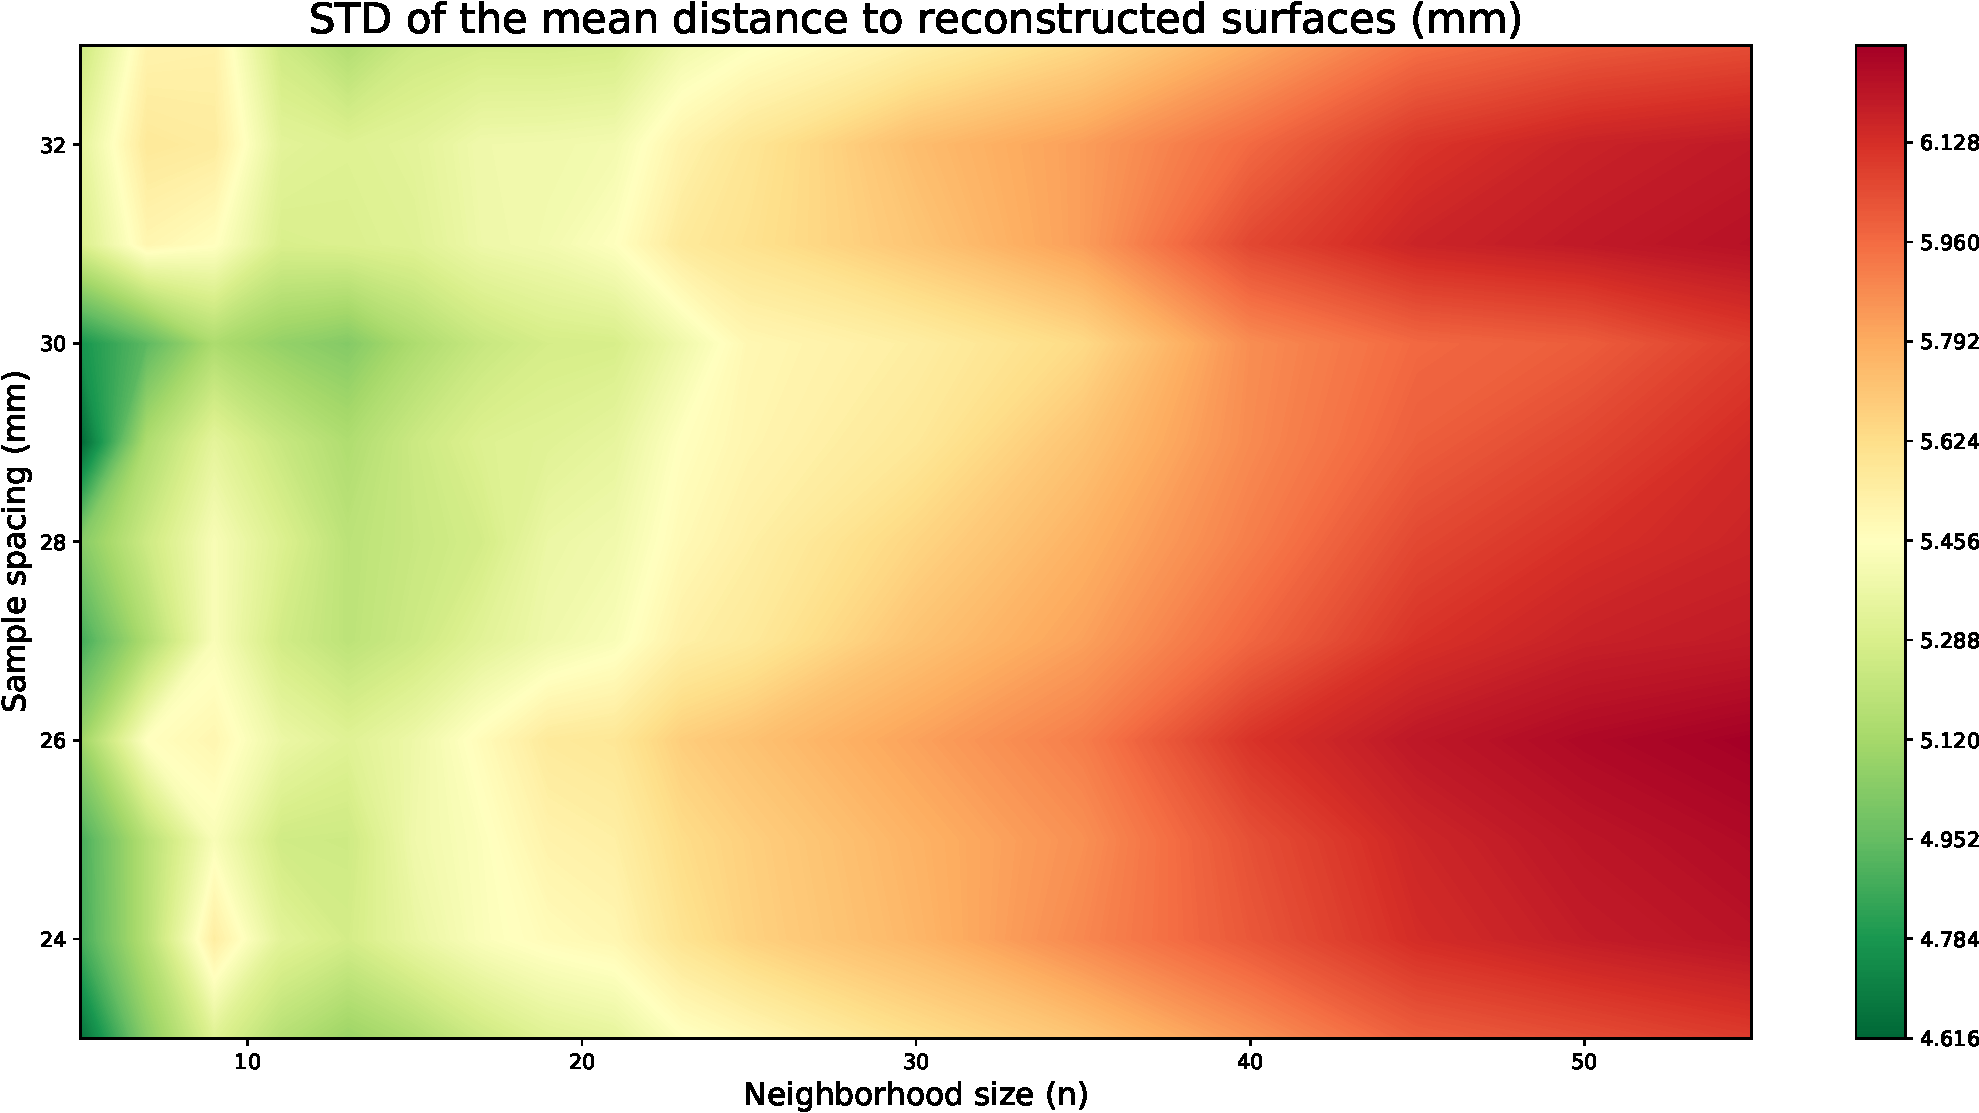
\includegraphics[width=0.9\textwidth]{gridSearchResultSTDCrop}
  \caption{This contour plot shows the STD of the mean distance calculated over 10
    differently sampled point collections. All point collections represent the
    surface of the same liver phantom.}
  \label{fig:gridSearchResultSTD}
\end{figure}
By simply summing up the mean and the standard deviation, one finds that the
optimal parameters for the tested surface samplings are 13 for the neighborhood
size and 30 mm for the sample spacing.
\section{Tumor Segmentation}
\label{sec:tumorSegmentation}
The flow diagram in figure \ref{fig:ThirdFlowChart} helps to understand the
following explanation of the creation of a tumor 3D model.
To create a 3D model of a tumor, the surgeon has to freeze an ultrasound image
such that the real tumor center is visible on this image. To find the location
of the tumor's center, the surgeon locates the tumor with the
ultrasound. Then he freezes the ultrasound image that cuts through the middle of
the tumor. The 6D pose of that ultrasound image is stored and the image is
passed to the next step.

Most tumors have roundish shapes. and a sphere is the easiest
geometrical shape that can be used to approximate a tumor's real shape. To
define a sphere two components are needed: the location and the radius of the
spere.

To get more information about the tumor, the tumor on the freezed image has to be segmented. This
segmentation is done semi automatically. That means the surgeon has to
roughly initialize the segmentation manually and then the graph cut algorithm
implemented by openCV will segment the the tumor. From the resulting
segmentation shape, the tumor center and radius are estimated. The center
corresponds to the mean of the segmented boarder pixels and the radius is the
mean between the largest and the shortest distance from the boarder pixels to
the estimated center pixel. By using the 6D pose corresponding to the ultrasoud
image used for the segmentation, the center pixel gets transformed into the
tracking camera coordinate system. Finally the sphere that approximates the
tumor can be drawn into the same coordinate system as the liver surface.
\begin{figure}[H]
  \centering
 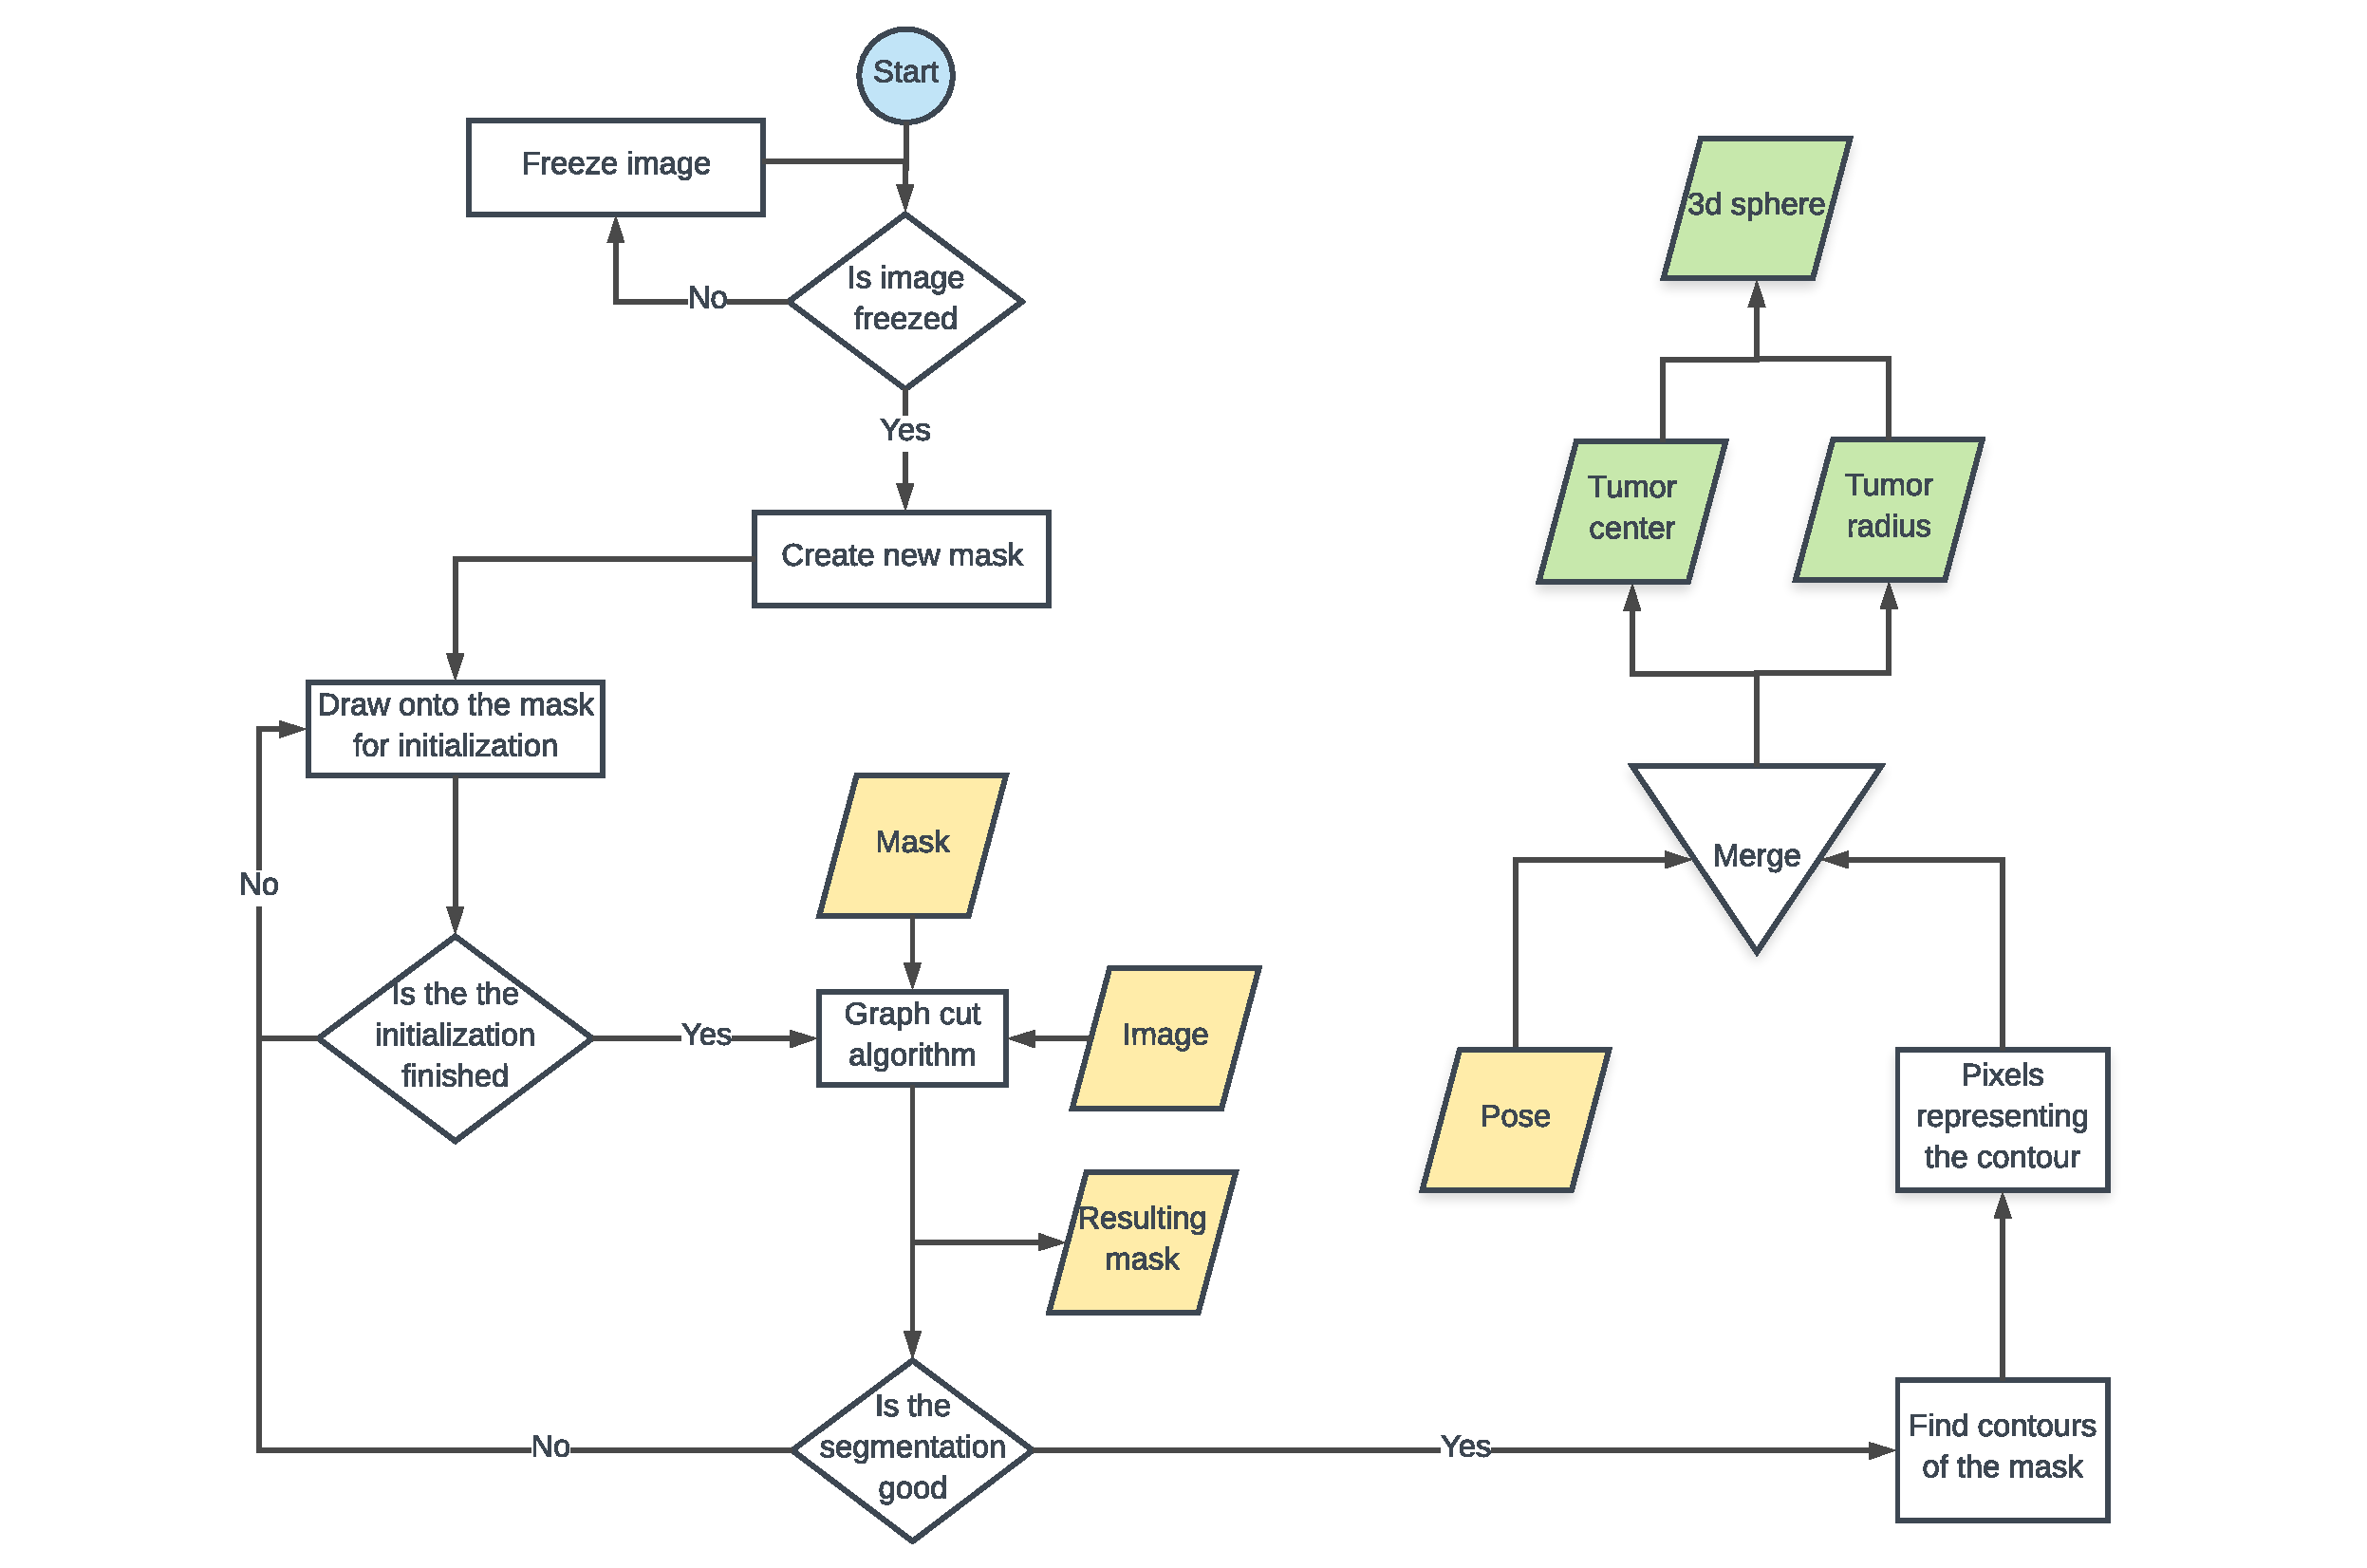
\includegraphics[width=1.2\textwidth]{ThirdFlowChart}
  \caption{The way of the image and its pose if the surgeon is scanning the
    surface.}
  \label{fig:ThirdFlowChart}
\end{figure}

\subsection{Initialization method}
As explained in section \ref{sec:tumorSegmentation}, the segmentation of the
tumor has to be initialized manually. This is done by drawing onto an
initialization mask. The surgeon draws two circles onto the mask. After clicking in the middle of the tumor, two
circles are drawn onto the mask. An orange
circle for the pixels that should be looked at to find the boundary of the
tumor (Figure \ref{fig:InitializeGraphCut}). And a red circle to color pixels surely
originating from the tumor. Most of the time the two circles need to be
increased or decreased in size. This is done by clicking the plus or minus
buttons. Both circles are changed at the same time. The position can be changed
by using the arrow buttons. As soon as the surgeon is satisfied, he confirms the
initialization and the created initialization mask is passed to the segmentation algorithm.
\begin{figure}[H]
  \centering
  \minipage{0.62\linewidth}
  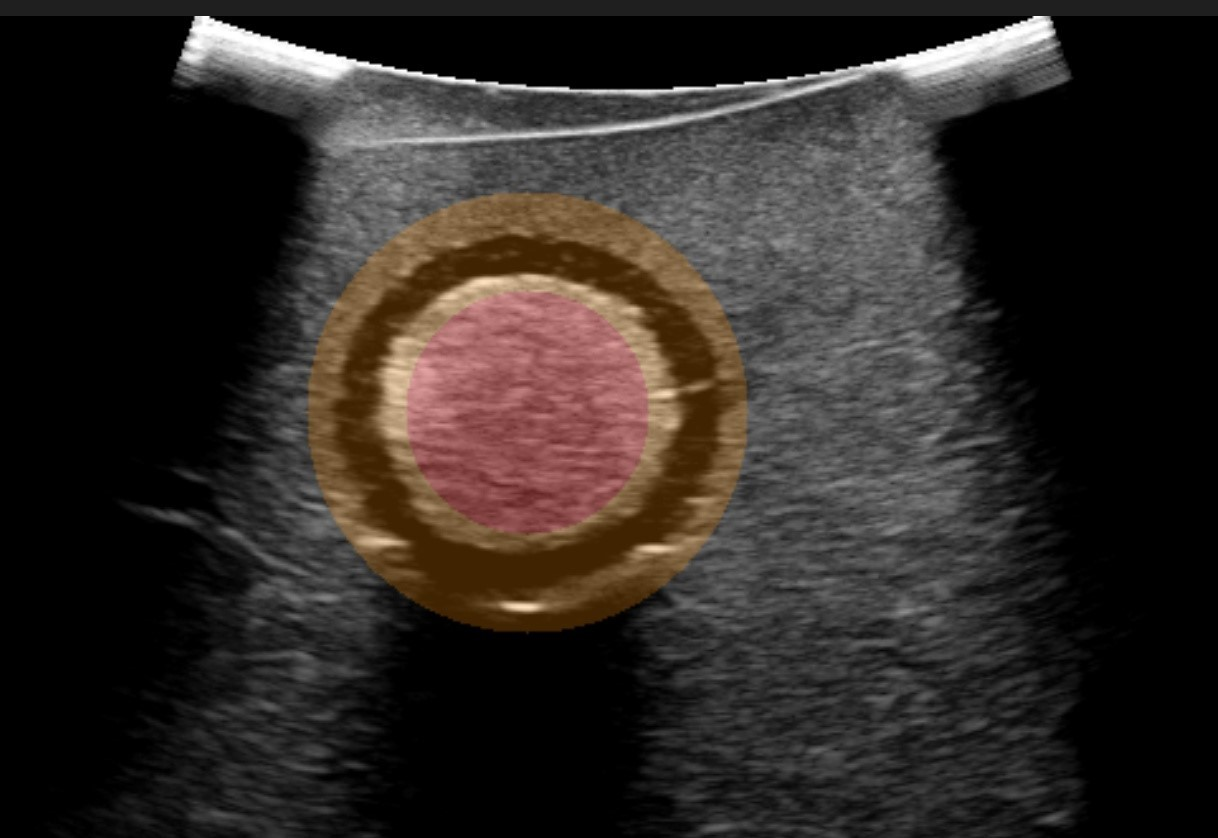
\includegraphics[width=\linewidth]{InitializationDrawing}
  \endminipage
  \hfill
  \minipage{0.32\linewidth}
  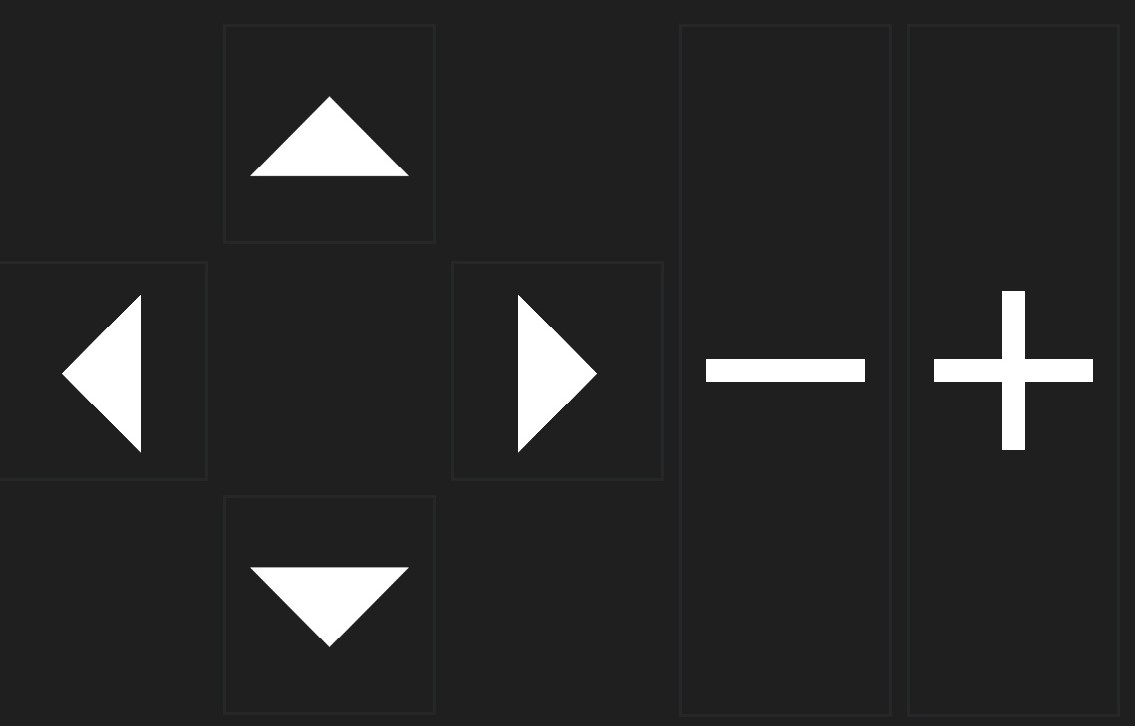
\includegraphics[width=\linewidth]{InitializationControls}
  \endminipage
  \hfill
  \caption{On the left side: Initialization drawing for the segmentation of the
    tumor. Red the pixels which are tumor pixels. And orange the pixels that are
    from the tumor or the background. The not colored pixels represent
    background. On the right side: Controls to manipulate the initial segmentation.}
  \label{fig:InitializeGraphCut}
\end{figure}

\subsection{Graph cuts}
For the segmentation a graph cuts algorithm is used. This algorithm treats
pixels as set of nodes connected in a graph (Figure
\ref{fig:graphCutsExplanaition}). Foreground and background are initialized by
selecting parts in the image.
% Some pixels have to be initialized
% as foreground and background.
Pixels labeled foreground belong to the source and
background labeled ones to the sink. The nodes (pixels) are connected to their
neighbors, the source, and the sink by
edges whose weights are defined as follows:
\begin{itemize}
  \item Node to source $\rightarrow$ Probability of the node to belong to the source (foreground)
  \item Node to sink $\rightarrow$ Probability of the node to belong to the sink (background)
  \item Node to adjacent node $\rightarrow$ Similarity measure to its neighboring node. 
\end{itemize}
A weight of an edge to adjacent node depends on the similarity between pixel intensities.
The edges between adjacent nodes, initialized to the same label, have an
infinitly high weight \cite{wiki:MaxFlow}.

After calculating all the weights in the graph, it has to be cutted in order to
create a segmentation. All pixels not assigned already in advance foreground or background will get assigned by
cutting the graph. The segmentation is obtained in form of a min-cut
\cite{Bagci2016} in which edges are removed to separate source and sink, and sum of their weights is
minimized.
% This means one separates the
% source from the sink by removing edges. All weights of the removed edges have to be summed up.
% The sum should be as small as possible and still separate the two from each
% other.
This way you can find a group of foreground and background pixels.
\begin{figure}[H]
  \centering
  \minipage{0.10\linewidth}
  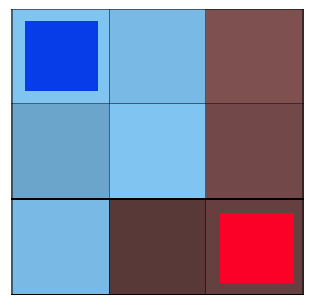
\includegraphics[width=\linewidth]{GraphCuts0} 
  \endminipage
  \hfill
  \minipage{0.22\linewidth}
  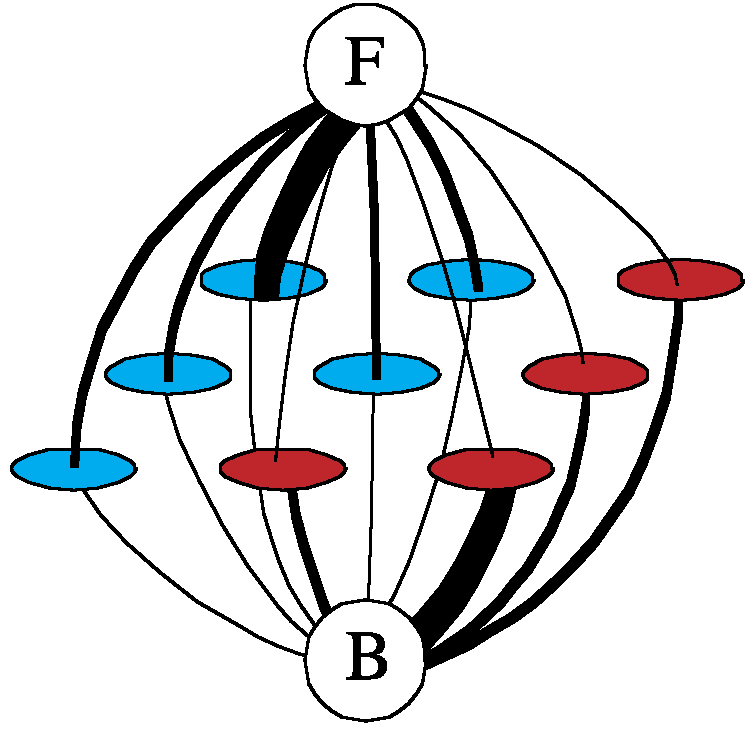
\includegraphics[width=\linewidth]{GraphCuts1} 
  \endminipage
  \hfill 
  \minipage{0.22\linewidth}
  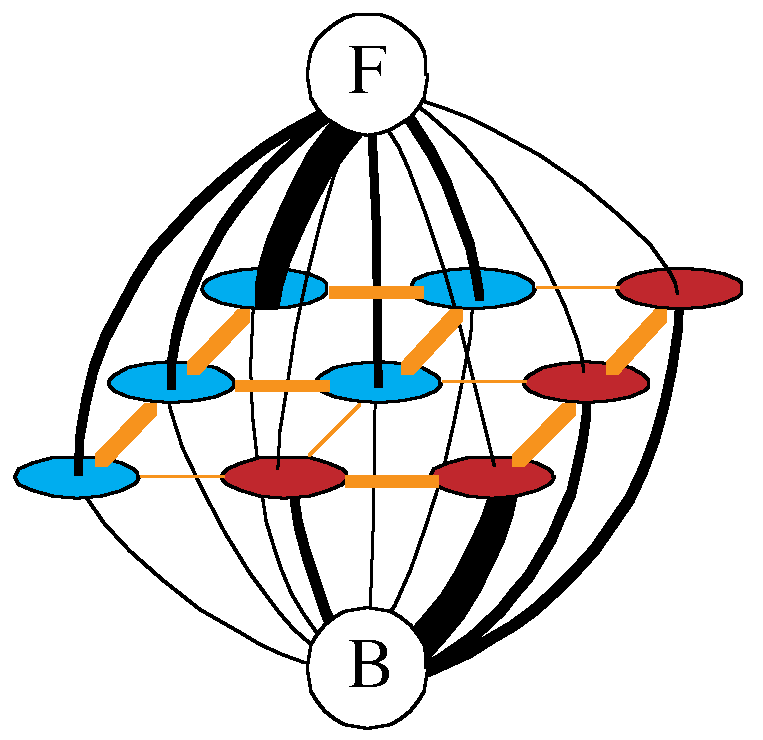
\includegraphics[width=\linewidth]{GraphCuts2} 
  \endminipage
  \hfill
  \minipage{0.22\linewidth}
  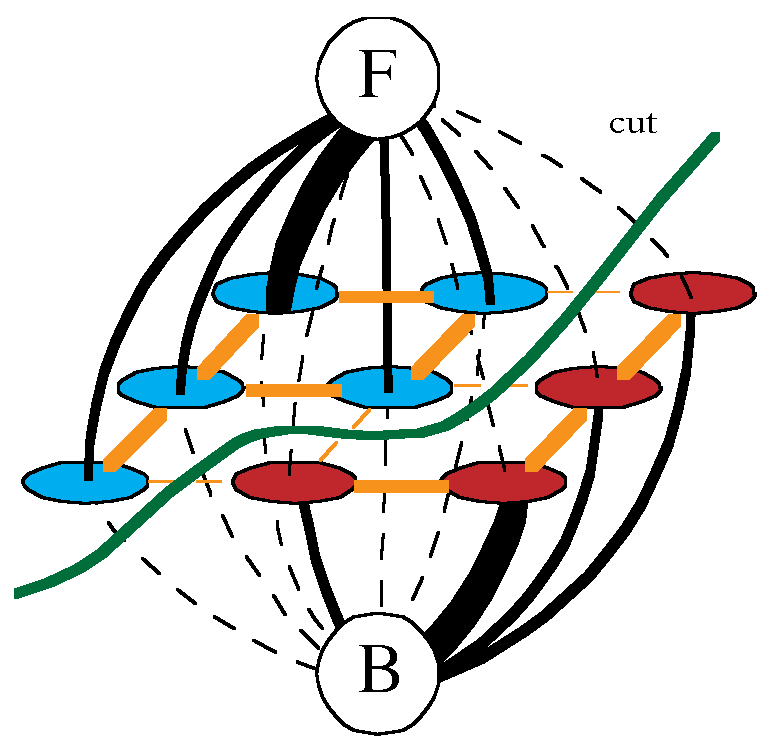
\includegraphics[width=\linewidth]{GraphCuts3} 
  \endminipage
  \hfill
  \minipage{0.22\linewidth}
  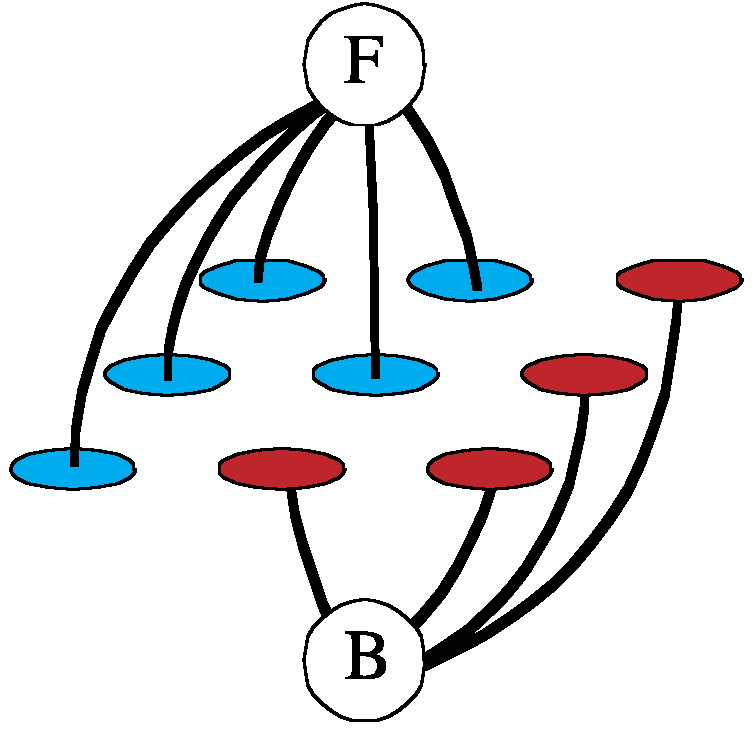
\includegraphics[width=\linewidth]{GraphCuts4} 
  \endminipage
  \hfill
 \caption{From left to right the steps of a graph cut segmentation. The first
   image shows the nine pixels to separate into foreground and background. A
   clear blue and a clear red drawing onto two pixels indicate the initialized
   foreground and background. The
   second image ilustrates the probabilities of each pixel belonging to the
   foreground or the background. The third image shows the edges between
   neighboring pixels in orange. The fourth image shows the edges to be cut as
   dashed lines. Finally the last image shows the result for foreground and
   background \cite{Bagci2016}.}
  \label{fig:graphCutsExplanaition}
\end{figure}

\section{Resection Planning}
The 3D models of the liver and the tumor are created. In this section we will
explain how the resection plane is calculated and displayed in the 3D scene. In
order to make better planning possible, the nearest point to the tumor center on
the surface of the liver must first be determined. To find this point, the
\textit{vtkCellLocator} class is used. This class has a function that can be
used to find the nearest point on a surface to a given point and the distance
between them. The found point and distance together with the polygonal data of
the liver surface, tumor, value for the safety margin, and the desired resection
shape are then passed into the resection calculator (Figure
\ref{fig:FourthFlowChart}).

The resection calculators task is to create a resection plane under the given
conditions and to represent it in the 3D model. It also shows the safety margin taken
into account as a sphere around the tumor. In addition, also a help line is displayed
on the liver surface to show where the surgeon could start the resection.
\begin{figure}[H]
  \centering
 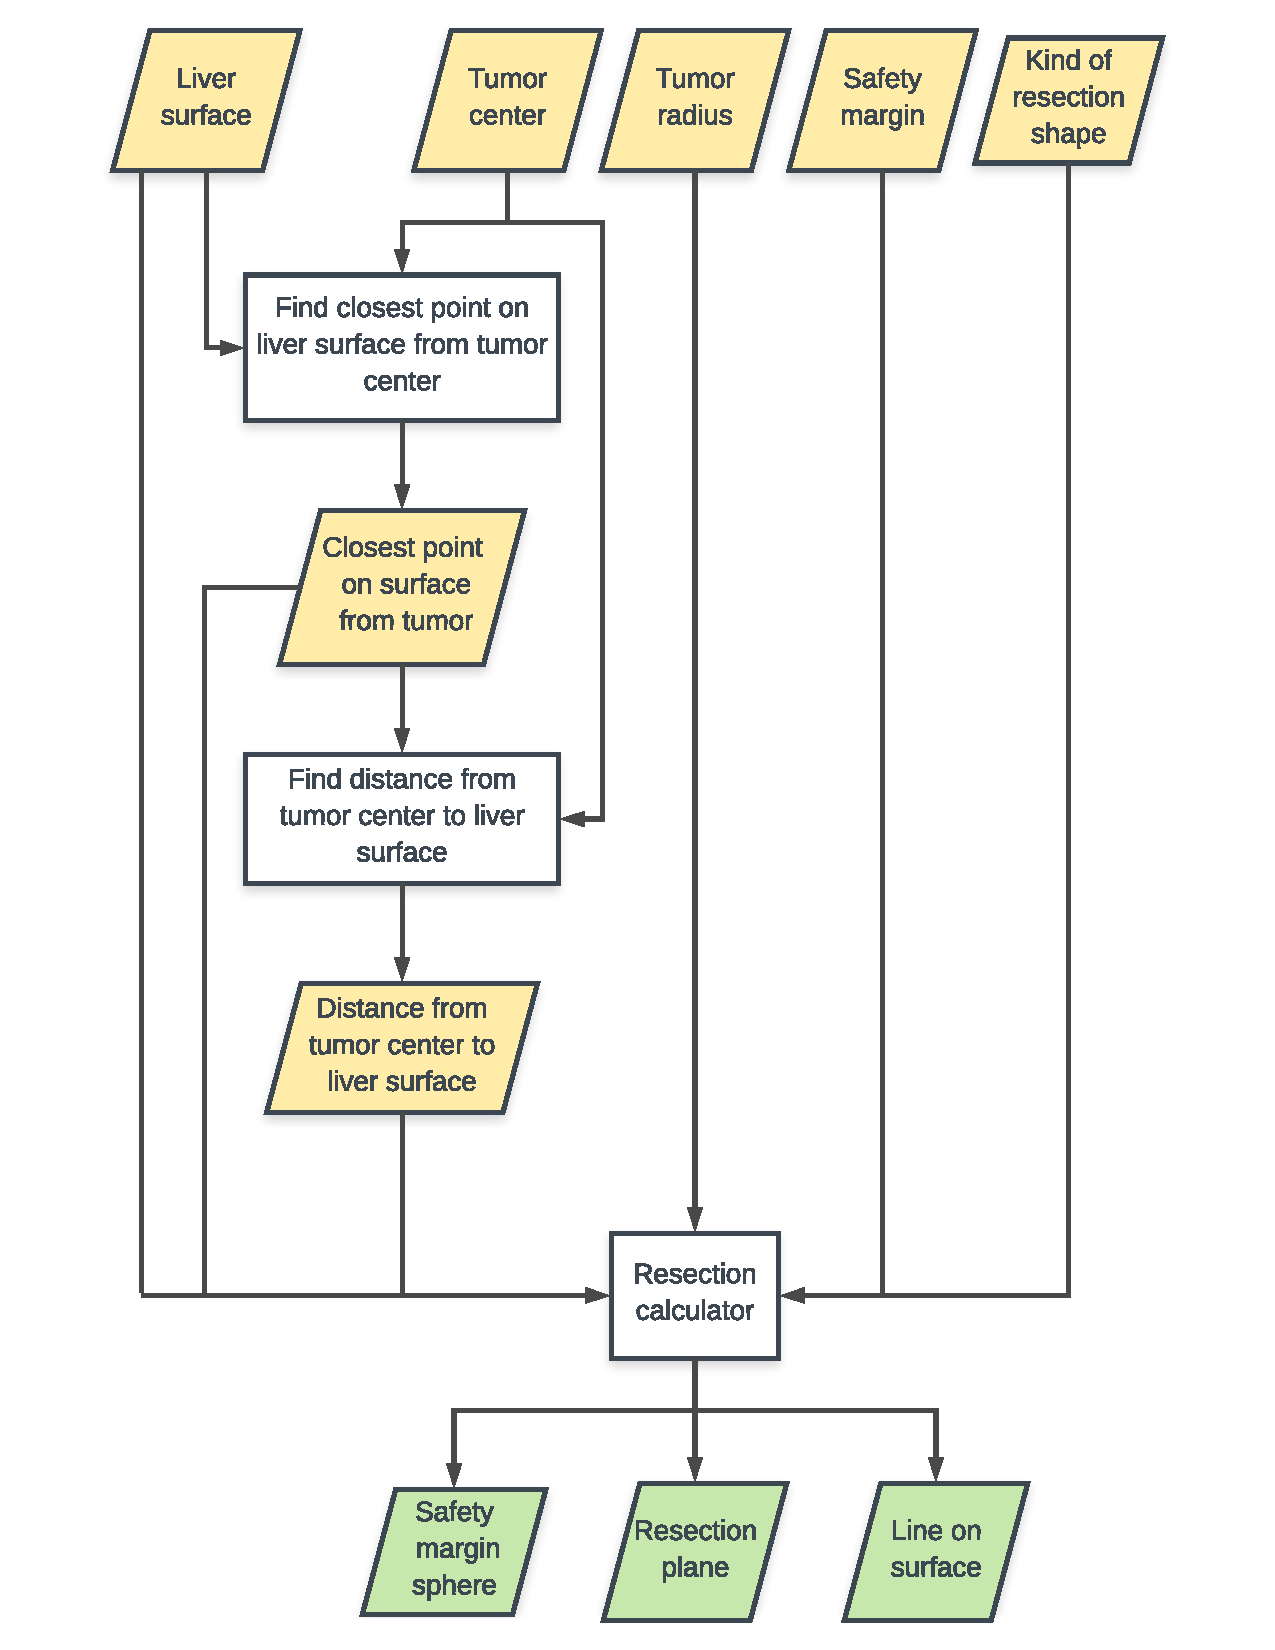
\includegraphics[width=0.65\textwidth]{FourthFlowChart}
  \caption{This flow chart shows the data flow to and from the resection calculator.}
  \label{fig:FourthFlowChart}
\end{figure}

\subsection{Cone fitting around tumor}
In order to keep as much healthy tissue as possible and still remove the tumor
while maintaining the necessary safety margin around the tumor, the resection
plane is recalculated for each tumor. Depending on the distance (d) between tumor
center (C) and liver surface the angle $\alpha$ varies between 10° and 30°. For
tumors with a distance less than 10 mm the angle is fixed to 30° and for
distances larger than 30 mm the angle is fixed to 10°. The direction of the cone
is defined by the vector from the tumor center to the nearest point (P) on the
surface. After constraining the cone to be tangential to the sphere of the
safety margin on both sides, the position of the cone apex (A) can be calculated. By
additiaonally forcing the cutting of the cone tangential to the sphere of the
safety margin, the length of the cone is limited towards the apex. The base of
the cone is defined to be 10 mm further away from the tumor than the surface
point. Finally we have the shape, size and position of the cone that leads to a
tissue sparing resection of the given tumor.
\begin{figure}[H]
  \centering
 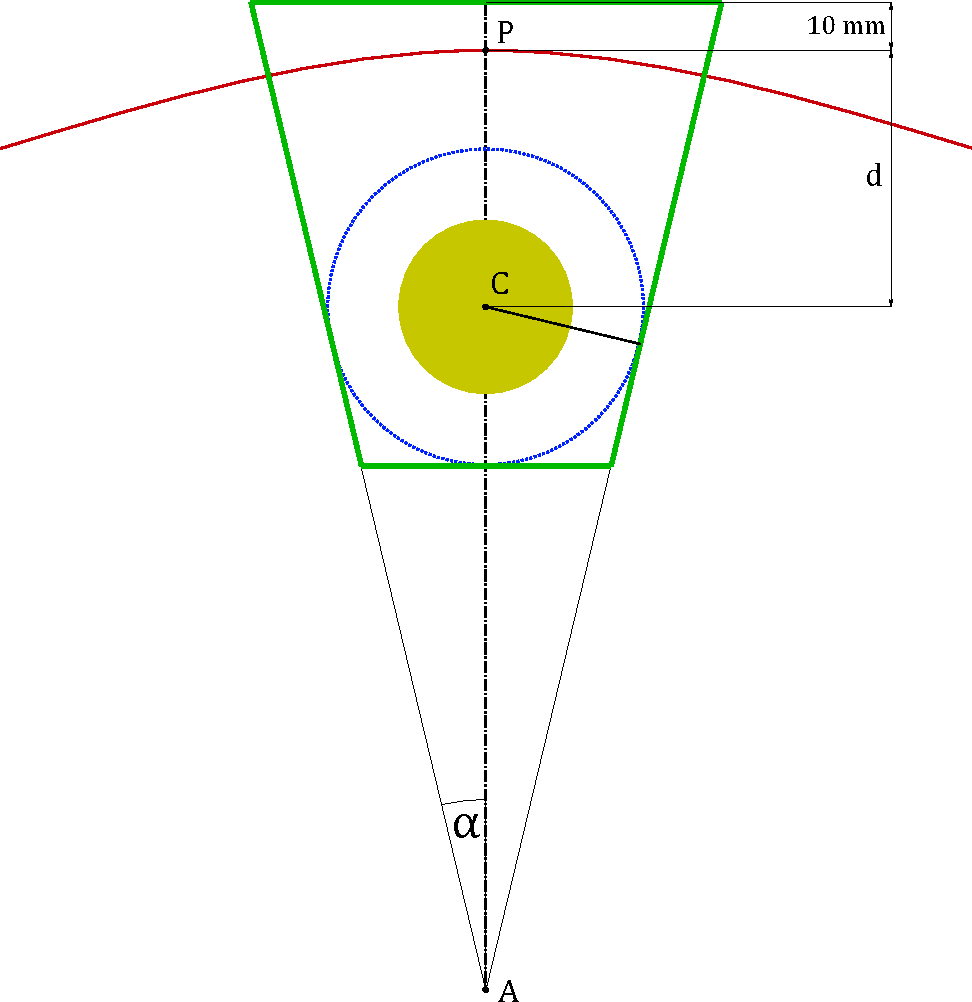
\includegraphics[width=0.5\textwidth]{ConeFittingGeometry}
  \caption{The geometrical shape of the resection plane (green) after fitting it
  around the safety margin (blue). The angle $\alpha$ depends on the distance (d)
  between the tumor center (C) and the closest point (P) on the liver surface to
  it. The position of the apex (A) can be calculated after constraining the
  safety margin to be tangential to the sides of the cone.}
  \label{fig:ConeFittingGeometry}
\end{figure}

\section{Visualization for navigation}
The visualization of the
previously created, virtual, assisting, 3D models to the surgeon should make the intervention
safer or even improve it. We use a 3D screen to show the 3D scene. This
makes it easier for the surgeon to move the surgical tools while looking at the
model.
Because surgeons need the ultrasound device a lot during liver resections, it
makes sense to combine the 3D models with the ultrasound image. 
% To help the surgeon navigate during the intervention, t
\subsection{Ultrasound overlay}
By blending the contours of all visible models (except the liver surface) which cut the image plane,
with the live ultrasound image, the 3D models become visible on the ultrasound
image (Figure \ref{fig:cutterExample}). Figure \ref{fig:FifthFlowChart} explains how an image and its
corresponding pose are used to cut the 3D scene and blend the contours with the
live image. First, the pose is used to check if the image cuts an object in the
scene. This is done with the \textit{vtkCutter} class. This class can cut
through a 3D object with an implicite function. The implicite function of an
image is a plane, and therefore simple to create by using the image pose. Because the
cutter can only return a binary mask of where it cuts an object, the cutter
has to check each object separately. Each time the returned mask from the cutter
is not empty, contour of the mask is found by using the openCV function
\textit{findContours}. The found contour is then colored depending on the color
of the cutted 3D object and added to the mask which will be finally blended with
the original image. If an object is fully transparent (not visible on the 3D
screen), then also the countour line will be fully transparent. The described procedure is performed for each new ultrasound image
during the navigated intervention. 
\begin{figure}[H]
  \centering
 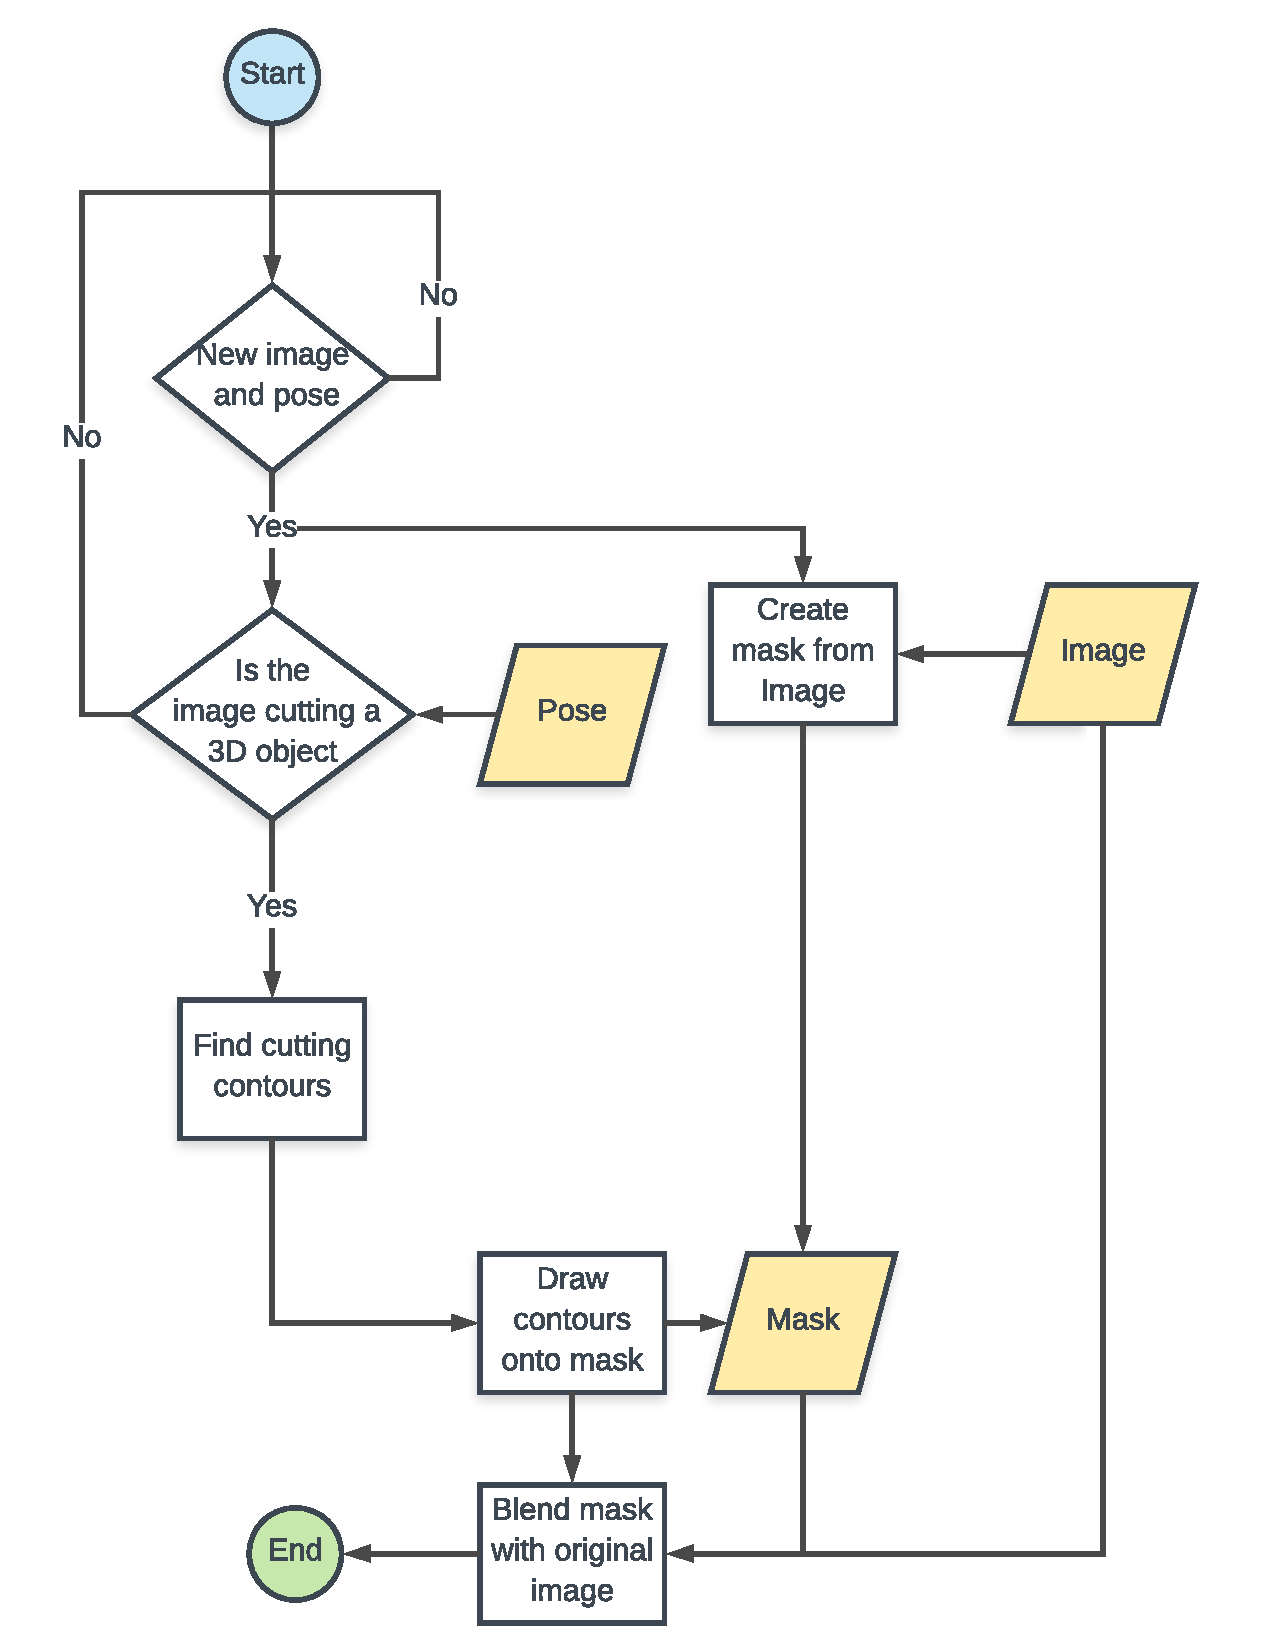
\includegraphics[width=0.5\textwidth]{FifthFlowChart}
  \caption{This flow chart shows the data flow to create the overlay of the 3D
    objects onto the live ultrasound images.}
  \label{fig:FifthFlowChart}
\end{figure}
\begin{figure}[H]
  \centering
  \minipage{0.48\linewidth}
  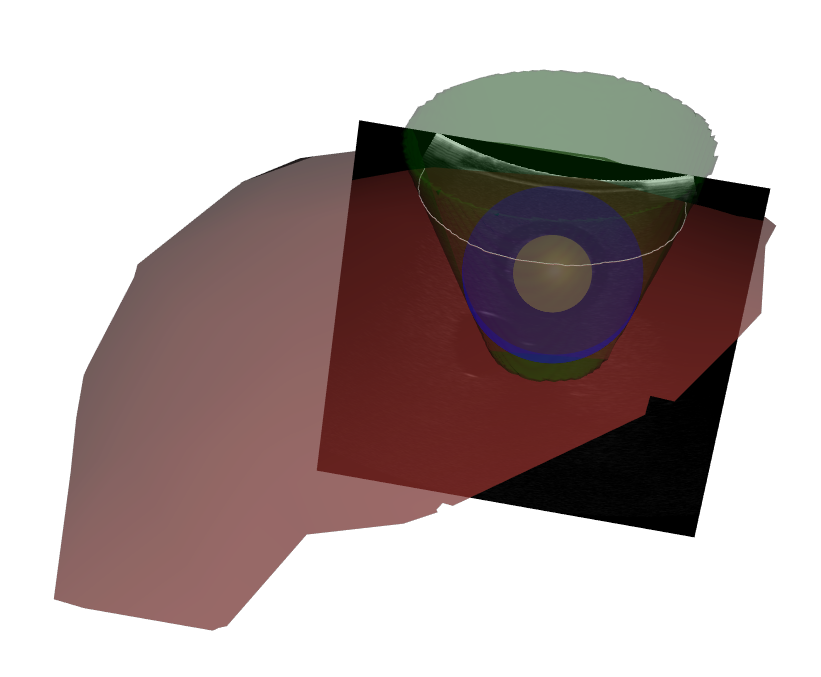
\includegraphics[width=\linewidth]{cutter3DView} 
  \endminipage
  \hfill
  \minipage{0.48\linewidth}
  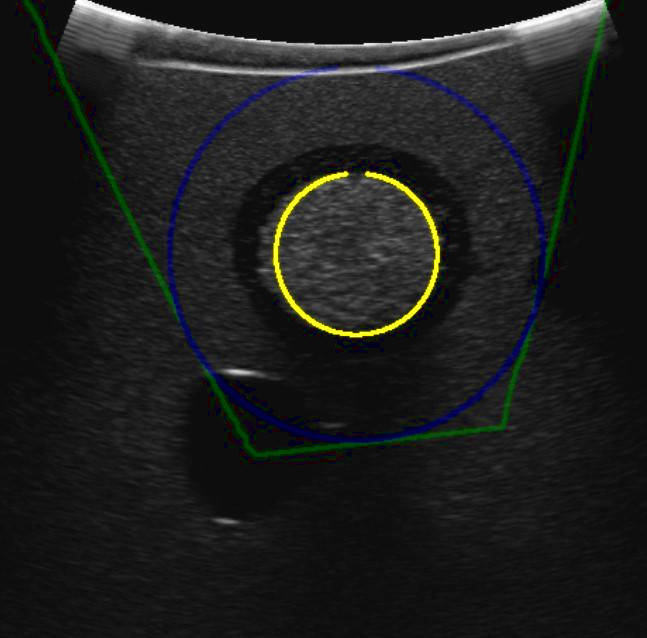
\includegraphics[width=\linewidth]{cutter2DView}
  \endminipage
  \hfill 
 \caption{On the left side is the 3D scene with the ultrasound image cutting
   through the tumor, safety margin and the resection plane. On the right side
   is the resulting cutting overlay on the live ultrasound image.}
  \label{fig:cutterExample}
\end{figure}
\subsection{3D model}
The complete 3D scene consists of the liver surface, approximated tumor sphere
in the size of the acutal tumor, sphere for the safety margin around the tumor,
resection plane and the line on the surface indicating the start of the
resection at the liver surface. Each model in the scene can be faded in or out
separately. The visibility of each model (except the liver surface) is toggeled on the touchscreen. The
visibility of a model can be toggled by clicking on the appropriate button on
the control touch-screen.
The model colors are the following:
\begin{itemize}
  \item Red $\rightarrow$ Liver surface
  \item Yellow $\rightarrow$ Tumor sphere
  \item Blue $\rightarrow$ Safety margin sphere
  \item Green $\rightarrow$ Resection plane
\end{itemize}
The liver surface, resection plane and the safety margin sphere are trasparent
such that one can see trough them.
\section{UI Concept}

%%% Local Variables:
%%% TeX-master: "MscThesis"
%%% End: